\section{Speaker Array: Measurement Results}
In order to investigate, how all the previous considerations about beamforming fare, when they are actually implemented, a series of measurements with a custom built speaker array has been conducted. A measurement protocol is given in \autoref{ax:directional_3}, as well as an overview over what individual measurements were conducted and what kinds of results were achieved. It is highly recommended to refer to the appendix when ambiguities occur while reading the following section.

\subsection{Beam Width}
As mentioned in \autoref{ch:intro}, for many practical applications it is desirable, that a sound sources radiates more sound into a particular direction then into other directions. Evenness over a given frequency range is often desirable. \autoref{fig:beamwidth_array} shows the measured relative pressure emission from the speaker array along the circumference of the speaker array in the frequency range of \SIrange{60}{300}{\hertz}. \autoref{fig:beamdwidth_array_off} shows the case, where all three speakers in the array play exactely the same signal, hence no beamforming is happening, wheras for \autoref{fig:beamdwidth_array_on}, beamforming was enabled. 
There is a significant difference in terms of directionality. Without beamforming, the sound emission from the array can be considered almost omnidirectional up to a frequency of approx. \SI{150}{\hertz}. At frequencies higher then this, an attenuation in the order of magnitude of \SIrange{3}{6}{\decibel} can be recorded near $\pm \SI{120}{\degree}$ in relation to the main axis of the array.\\
The picture drastically changes when beamforming is enabled. The \SI{-3}{\decibel} lobe width is within a range of approx. \SIrange{110}{150}{\degree} over the entire frequency range of \SIrange{60}{300}{\hertz}. The borders of the \SI{-6}{\decibel} and \SI{-9}{\decibel} lobes width are approximately parallel to the \SI{-3}{\decibel} lobes. The \SI{-9}{\decibel} lobe width is roughly \SI{220}{\degree} width a tendency to be wider at low frequencies and to become more narrow at frequencies higher than \SI{220}{\hertz}. For higher pressure drops the behaviour over the frequency range is less similar. Some ``trenches" at approx. \SI{\pm 150}{\degree} e.g. between \SI{120}{\hertz} and \SI{190}{\hertz}, exceeding a pressure drop of \SI{24}{\decibel} compared to the main axis. These correspond to the spikes in some of the polar plots in \autoref{sec:meas_vs_theory}, e.g. \autoref{fig:200_hz_polar_result}. It is also visible, that the pressure around \SI{\pm 180}{\degree} changes quite significantly over the frequency range. This corresponds to a variation in rear lobe pressure on the polar plots in \autoref{sec:meas_vs_theory}, e.g. \autoref{fig:150_hz_polar_result} and \autoref{fig:300_hz_polar_result}.
Measured pressure does not behave perfectly symmetrical in relation to the \SI{0}{\degree} axis, e.g. at approx. \SI{200}{\hertz} and approx. \SI{\pm 150}{\degree}. This might indicate some alignment issues during the measurement, meaning that the speakers~B and C might have not been positioned perfectly parallel to the main axis of speaker~A.\\
From the behaviour illustrated in \autoref{fig:beamdwidth_array_on} it can be concluded, that the speaker array is suitable for a typical audio playback setting, where the audience is placed in an angle close to the main axis of the array. Because the attenuation is relatively even over the investigated frequency band, meaning that listeners within an angle of approx. \SI{\pm 90}{\degree} are exposed to sound with all frequencies within the investigated range being at approximately the same level.

\begin{figure}[h]
	\centering
	\begin{subfigure}[c]{\textwidth}
		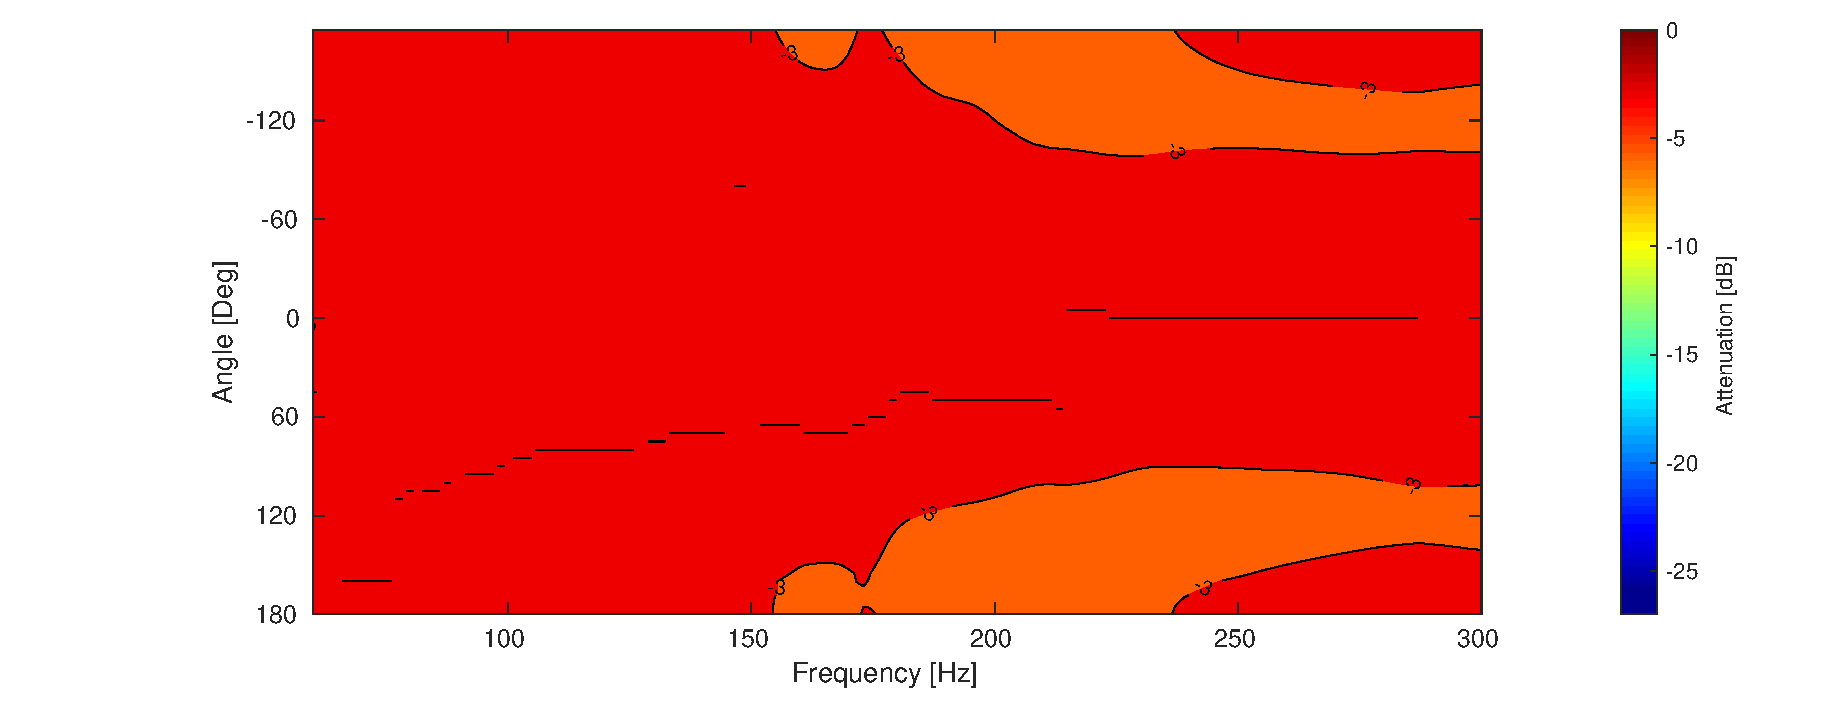
\includegraphics[width=1\textwidth]{beamwidth_disabled.eps}
		\subcaption{Speaker array, beamforming disabled.}
		\label{fig:beamdwidth_array_off}
	\end{subfigure}\\
		\begin{subfigure}[c]{\textwidth}
		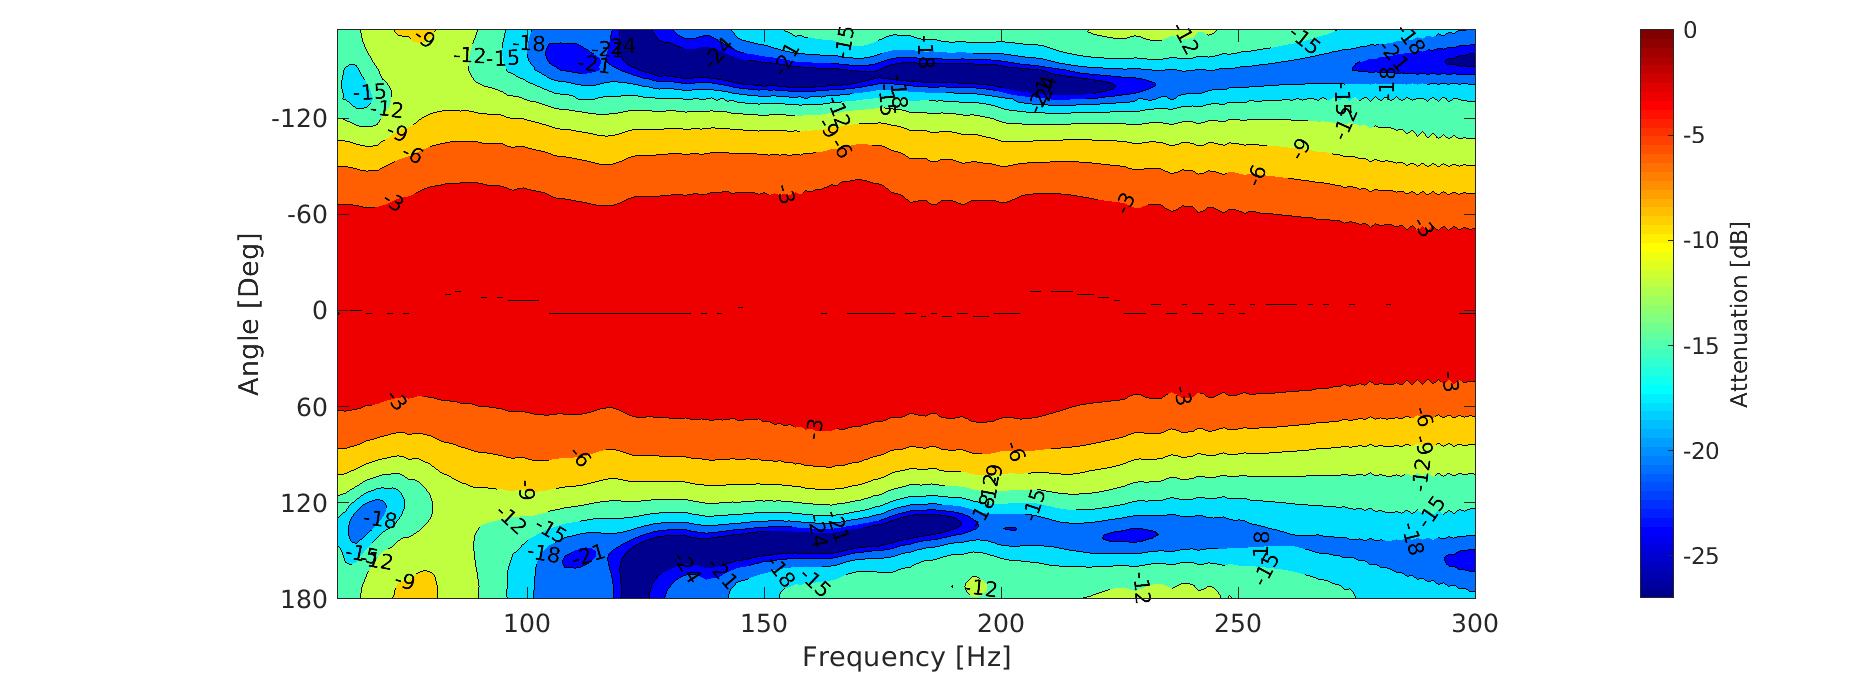
\includegraphics[width=1\textwidth]{beamwidth_final.eps}
		\subcaption{Speaker array, beamforming enabled.}
		\label{fig:beamdwidth_array_on}
	\end{subfigure}\\
	\caption{Contour plots of the relative level over frequency and angle, based on data from the measurements in \autoref{ax:directional_3}}
	\label{fig:beamwidth_array}
\end{figure}